%\dropchapter{0.4in}
\chapter{The CMS experiment at CERN's accelerator complex} \label{chp:CERN}
%\epigraphhead[70]{\epigraph{\textit{If I could remember the names of all these particles, I'd be a botanist.}}{Enrico Fermi}}
%\undodrop

The Standard Model of elementary particle physics, for which its main successes and shortcomings has been discussed extensively in Chapter~\ref{chp::SM}, has proven to result in very precise predictions. However it is only acknowledged as an effective theory up to an energy scale of about 1 $\TeV$. Physics beyond this energy range is studied with specific high-energetic particle colliders including, for example, the Large Hadron Collider (LHC) located at CERN (European Council for Nuclear Research) near Geneva. The LHC provides proton-proton collisions at a record-breaking energy and is currently the world's most energetic particle collider.\\
Many different experiments surround the Large Hadron Collider each with a specific physics goal ranging from general high-luminosity physics to dedicated plasma-studies and even long-lifetime neutrino interactions (and even medical ...??).
In this chapter attention will mainly be devoted to the CMS experiment, which is the LHC general-purpose experiment used for collecting data processed within this thesis.

\section{The Large Hadron Collider}
The need for a particle collider with the (enormous) dimensions of the LHC was driven by a quest to understand the nature of the electroweak symmetry breaking, for which the Higgs mechanism is presumed to be responsible, and investigate the $\TeV$ scale.
\\
\textit{\textbf{Useful to mention here again?}}
\\

When the design of the LHC machine was approved in 1994 it was decided to reuse the existing 26.7 $\km$ Large Electron Positron (LEP) tunnel, previously excavated in the 1980's and positioned between 45m and 150m below the Earth's surface.
Avoiding the excavation of a new tunnel was a huge cost-saver but presented some stringent limitations on the machine's design. For example the space limitation in the tunnel compelled the use of so-called ``twin-bore'' magnets where both proton rings are contained within a single magnet structure.
\\
The LHC is designed to provide proton-proton collisions with a beam energy of 7 $\TeV$ each, resulting in a centre-of-mass energy of 14 $\TeV$. This is a seven-fold energy increase compared to the previous most energetic particle collider: the Tevatron~\cite{} which yielded proton-antiproton collisions between 19.. up to 2014 (?). In order to reach these extreme energy conditions the LHC exploits the presence of the extensive accelerator complex present at CERN to increase the beam energy gradually. This adopted accelerator sequence is denominated as the injection chain of the LHC and will be discussed in detail further in the text.
\\
When the proton beams are circulating within the LHC at the desired beam energy they can be forced to collide head-on in the dedicated interaction regions where beam crossings are provided. Of the eight interaction regions existing in the LEP tunnel only four have been equipped with particle detectors for the LHC run. The ATLAS~\cite{} and CMS~\cite{} experiments are the two largest ones and are intended as general-purpose detectors studying a broad range of high-luminosity\footnote{Maybe best to use other word than luminosity since it will only be explained afterwards ...} physics while the ALICE~\cite{} and LHCb~\cite{} experiments search for a specific type of physics interactions. The former one serves mainly as a heavy-ion detector while the latter one is dedicated to heavy-flavour physics.
\\
Within this thesis data collected at the CMS detector during the first era of data-taking has been analyzed, which started in March 2010 and continued until December 2012. These collisions did not take place at the design beam energy of 7 $\TeV$ but at a reduced energy of 3.5 $\TeV$ and 4 $\TeV$ for the 2010-2011 and 2012 data-taking, respectively. \textit{Maybe just put some of the main characteristics corresponding to this run to have similar information of all four parts!}

\subsubsection{LHC design, driven by the LEP legacy}
The design of the LHC project, approved in 1994 by the CERN council, is characterized by both the predefined ($\TeV$-scale) physics reach and the available infrastructure at the CERN accelerator complex.
The obligation to reuse the existing LEP tunnel introduced some additional challenges on top of the extremely high energy regime. 
\\
The decision to accelerate protons instead of electrons, as was the case for LEP, was led by the extremely high beam energy desired for the colliding partons. Less massive particles loose a significant amount of their energy due to synchrotron radiation when accelerated at high speed in an orbit while this is close to negligible for protons. With the velocities close to the speed of light foreseen at the LHC this energy loss would represent a limiting factor for the final energy reachable when accelerating electrons.
\\
\\
An important parameter of a particle accelerator is the luminosity $\mathcal{L}$, which represents the number of collisions that can be produced.
At the LHC the luminosity was designed to attain a record-breaking value of $10^{34}$ $\cm^{-2}$ $\s^{-1}$, corresponding to around 1 billion proton-proton interactions per second. Such a high rate of collisions is only feasible when the protons are confined into dense bunches and when multiple of these bunches circulate in the beampipe.
In order to reach this design luminosity the LHC should contain 2802 proton bunches with a separation of only 25 $\ns$ while each of these bunches consists of about $10^{11}$ protons.
\\
In order to fullfill these challenging conditions protons need to be produced in adequate amounts, a process which is not realizable for anti-protons. This is the prime motivation why the LHC yields proton-proton interactions, and not $p\bar{p}$ collisions as was done at the Tevatron.
%These challenging requirements are the main reason why the LHC yields proton-proton interactions instead of $p\bar{p}$ collisions at the Tevatron: anti-protons can not be produced in adequate amounts in order to end up with such high luminosities.
However the use of partons with the same electric charge introduces an additional challenge since two separate magnetic fields are required to bend the protons in opposite directions. For the LHC this lead to the development of twin-bore magnets containing two separate beam pipes and surrounding superconducting coils within the same mechanical structure. A schematic cross-section of such an LHC dipole magnet is given in Figure~\ref{fig::LHCDipole}.
\\
The relatively small circumference of the LHC tunnel combined with the extremely high velocity of the protons circulating compels the use of superconducting magnets. Although superconductivity was already used extensively in previous accelerators, the LHC (design) pushed the existing technology to a new level by operating at a record-breaking temperature of 1.9 $\K$ allowing the magnets to produce a magnetic field of 8.33 $\T$. Within the LHC 1232 of these dipole magnets exist which are responsible for bending the proton's trajectory.
\begin{figure}[h!t]
 \centering
 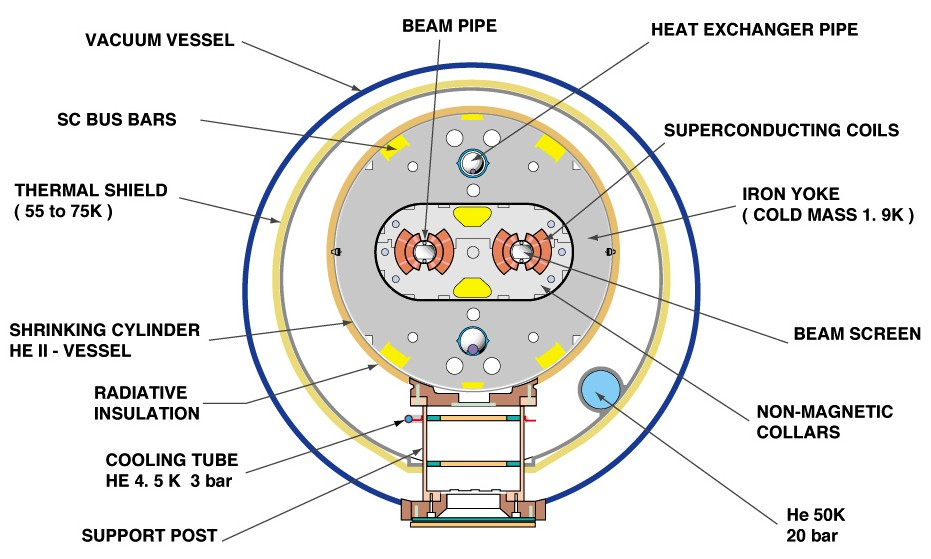
\includegraphics[width = 0.6 \textwidth]{Chapters/Chapter2_CERN/Figures/lhc-pho-1998-341.jpg}
 \caption{Cross-section of an LHC dipole magnet with the twin-bore design.}%Taken from http://cds.cern.ch/record/841539/
 \label{fig::LHCDipole}
\end{figure}

The tunnel of the Large Hadron Collider is not a perfect circle but consists of eight arcs and eight straight sections each with its specific functions. 
The arcs are responsible for preserving the circular orbit and contain the 15 $\m$ long dipole magnets.
The straight sections ensure that the beams remain aligned and do not drift apart by using specific quadrupole magnets. These type of magnets are able to squeeze the beam either vertically or horizontally and are also installed just before the different detectors where they provide an additional squeezing to increase the chances on a collision. A second role which is provided by these straight section is accelerating the beam with radiofrequency (RF) cavities.

\subsubsection{The LHC injection chain}
The LHC does not only reuse the existing LEP tunnel it also benefits strongly from the complete accelerator complex present at CERN in order to reach the record energy of 7 $\TeV$. 
The protons run through a series of interconnected linear and circular accelerators and are only passed on to the next in line once they attained the maximum speed possible for that specific accelerator. A schematic overview of the sequence used for the proton acceleration at the LHC is given in Figure~\ref{fig::LHCChain}.\\
The entire LHC injection chain originates from a box of hydrogen atoms from which protons are electrically stripped and directly accelerated to an energy of about 50 $\MeV$ by the Linac2.
From here they are injected into the first circular accelerator, the Proton Synchrotron Booster (PSB), until they reach an energy of 1.4 $\GeV$ and are energetic enough to be shot into the Proton Synchrotron (PS). Here they will circulate until they arrive at the maximum speed possible for the PS, which corresponds to an energy of 25 $\GeV$, and are inserted in the final pre-accelerating machine: the Super Proton Synchrotron (SPS). The SPS is responsible for accelerating the protons up to 450 $\GeV$ after which the LHC is capable of accelerating them further until the nominal energy of 7 $\GeV$, a process which takes about 20 minutes.

\begin{figure}[h!t]
 \centering
 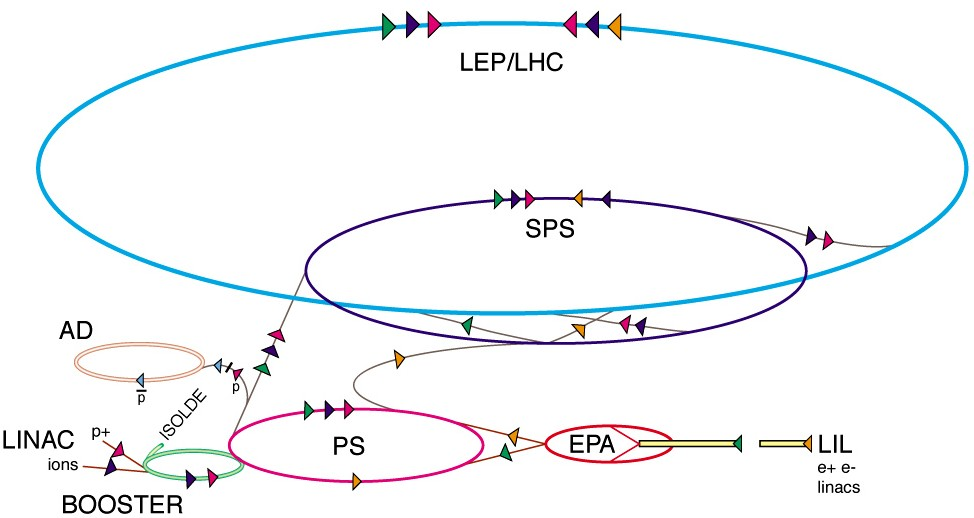
\includegraphics[width = 0.8 \textwidth]{Chapters/Chapter2_CERN/Figures/CERNAcceleratorComplex_Few.jpg}
 \caption{Overview with fewest detail}
\end{figure}

\begin{figure}[h!t]
 \centering
 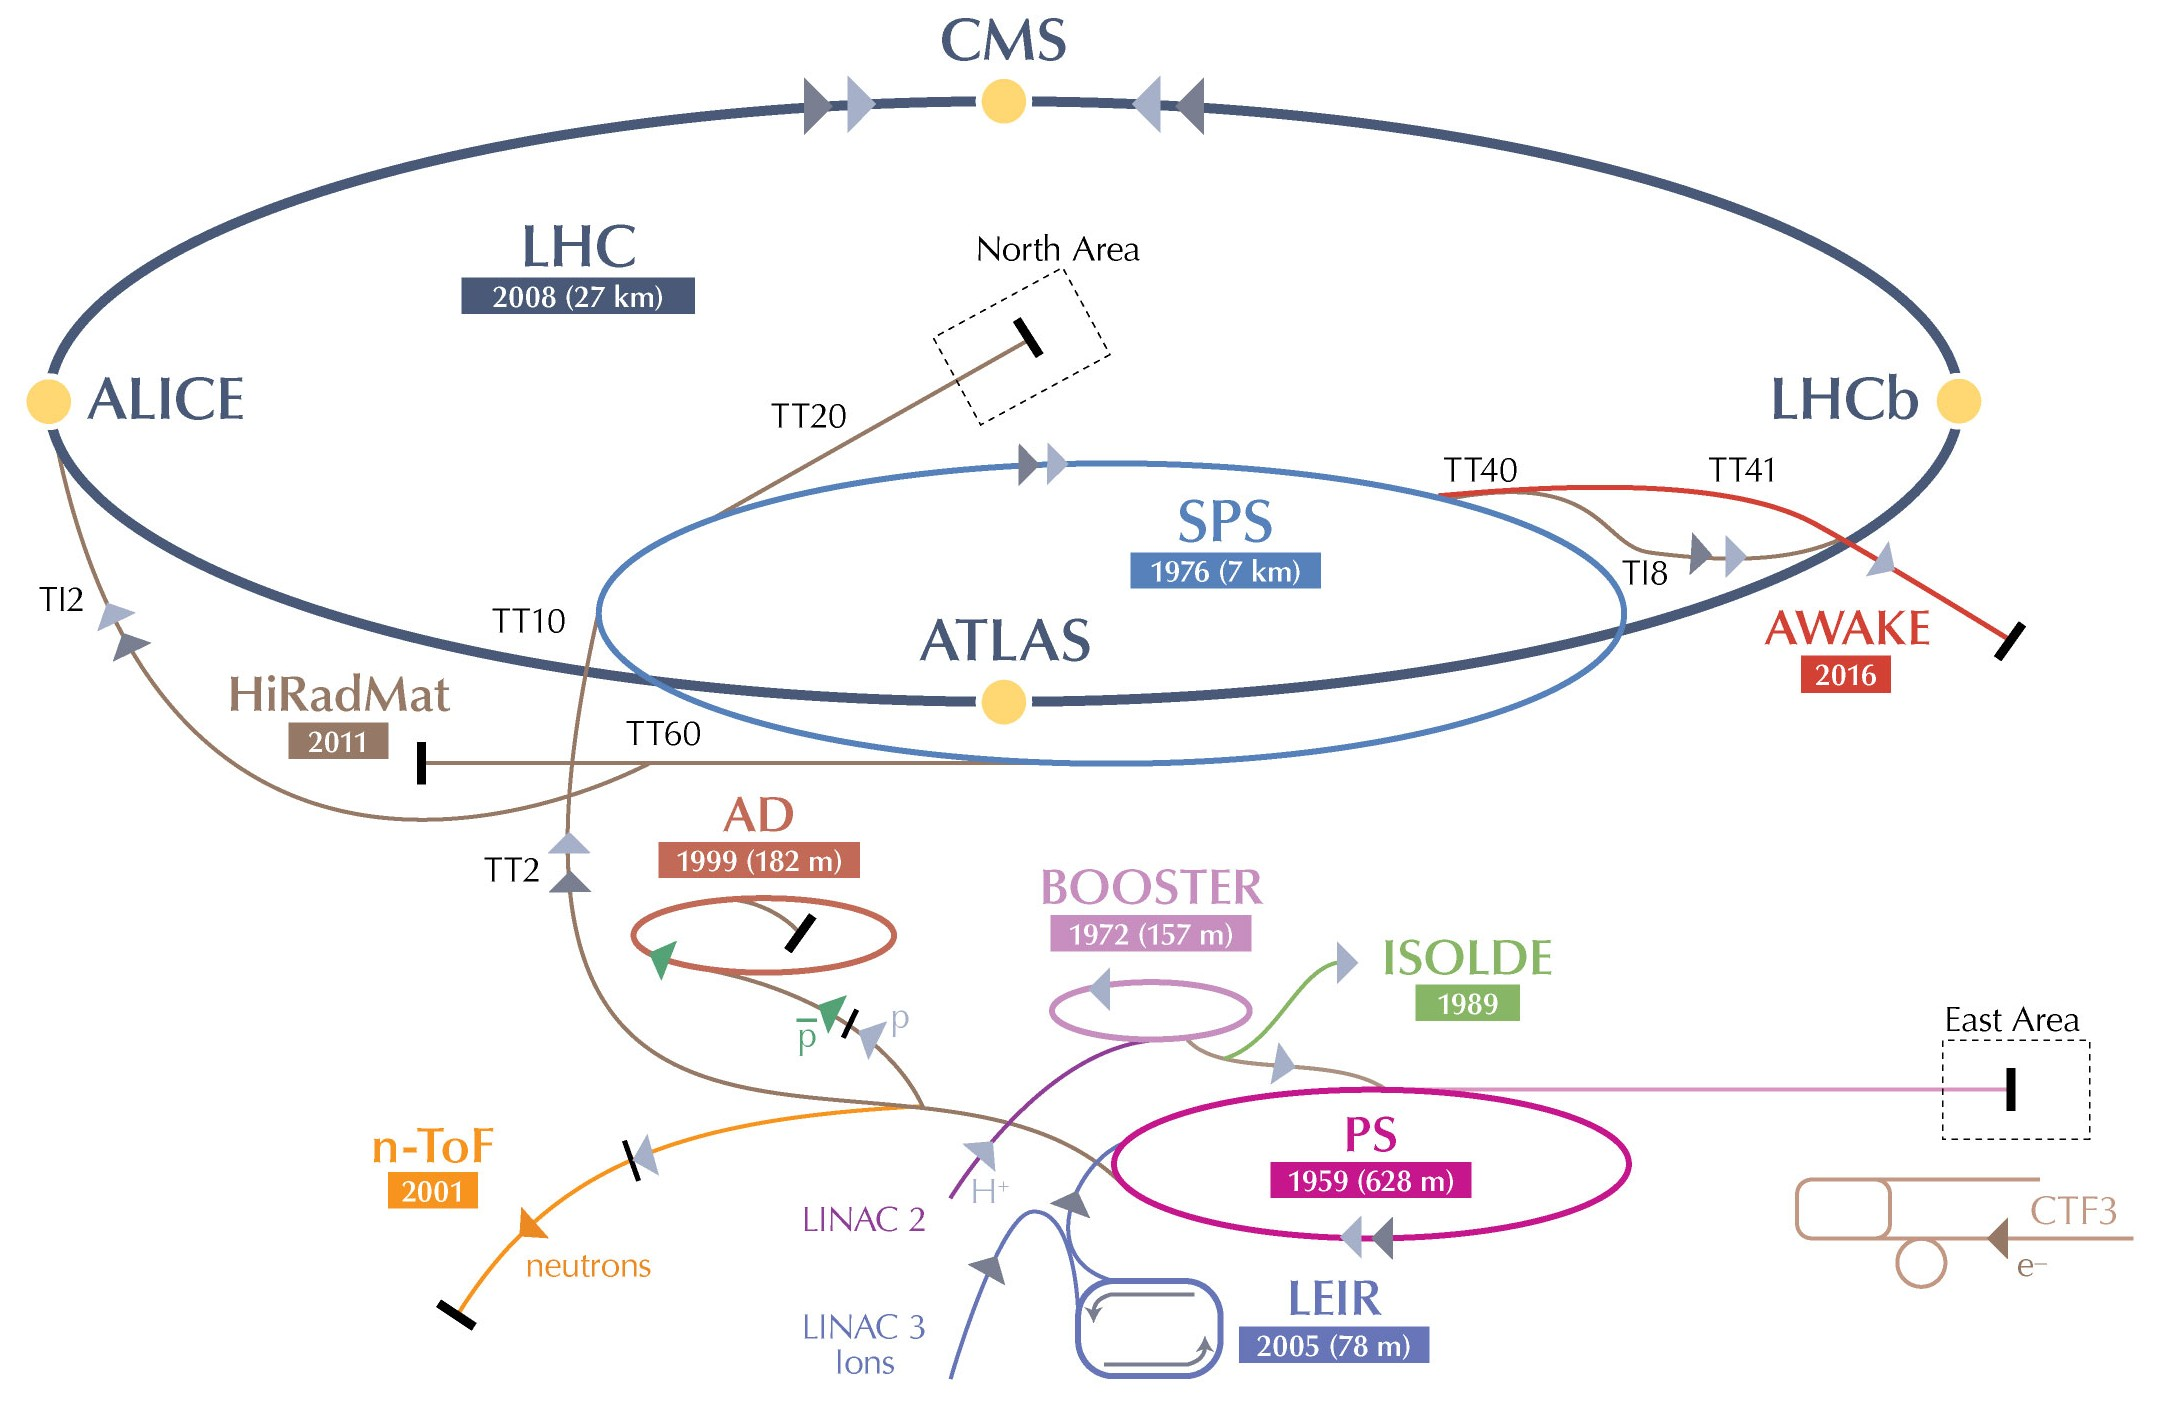
\includegraphics[width = 0.99 \textwidth]{Chapters/Chapter2_CERN/Figures/CERNAcceleratorComplex_Detail.jpg}
 \caption{Overview with most detail (seems to be less fine than in thesis Stijn)} \label{fig::LHCChain}
\end{figure}


The Large Hadron Collider does not simply collide individual protons but actually provides collisions between bunches of $10^{11}$ protons to ensure at least one proton-proton interaction during a single bunch crossing. The design of the LHC is optimized not only for providing $pp$ collision with a record-breaking beam energy, but also with the highest luminosity ever recorded. In order to satisfy this last requirement the LHC should contain multiple proton bunches in a so-called bunch train with the smallest separation possible between individual bunches, a technique also used in many older parton accelerators. 
However for the LHC this bunch separation, which specifies the time available between consecutive proton-proton interactions, has a nominal value of only 25 or 50 $\ns$, many times lower than currently adopted. \textbf{NOT GOOD!} (Maybe specify which value used for 8 TeV and 7 TeV)
\\
The formation of these proton bunches is provided by the RF cavities responsible for accelerating the protons and already starts during the first stages of the LHC injection chain. 
Radiofrequency cavities produce a resonant electromagnetic wave that oscillates at a given frequency and accelerates the protons up to an ideal energy since protons travelling too fast will undergo a deceleration while those arriving late will feel an additional push.
Hence inverting the electromagnetic field ensures that the protons become organized into discrete packets or bunches.
%and hence organize the protons into discrete packets or bunches. %, which is the reason why the protons get organized into large bunches.
%Inverting the electromagnetic field ensures that the protons will be accelerated up to an ideal energy since protons travelling too fast will undergo a deceleration while those arriving late will feel an additional push.
%The protons traversing such an RF cavity will feel the overall force and direction of the electromagnetic wave 
%Inverting the electromagnetic field ensures that the protons either get decelerated or accelerated whether they are faster or slower than the ideal proton energy for this resonant wave. Hence once the full energy is reached, this ideal proton will not feel any acceleration
%Due to the inversion of the electromagnetic field \underline{will the protons} either be decelerated or accelerated 
%Organizing the protons in bunches already starts during the first stages of the LHC injection chain and is provided by the RF cavities. These type of accelerating cavities 
%These proton bunches are produced during the first stages of the LHC injection chain and is taken care of by the use of RF cavities ....
%and the filling of the accelerator next in line already 
%is done as such 
%The creation of these proton bunches already starts in the first stages of the LHC injection chain and the filling of the next accelerator in line is done in such a way that the bunch trains are also created from the start.
\\
The RF cavities of the accelerators in the LHC injection chain are constructed such that each consecutive accelerator is capable of holding more bunches such that the bunch train can be expanded in a stepwise manner. This way the time needed to fill the LHC can be reduced significantly since the maximum number of bunches possible is accelerated and then passed on to the next accelerator in line. (\textit{so what does this mean, does the next accelerator has to wait until all the bunches are filled or is it capable to hold bunches with different speeds ???})

%Besides accelerating the protons this injection chain is also used to create the bunch structure which ... (benefit of these bunches)



%\textbf{\textit{How are the bunches formed??}} \\
%Seems to be caused by the harmonic oscillations of the Radiofrequency (RF) cavities which either accelerate or deccelerate protons such that they oscillate around the ideal energy and combine into bunches. (\textit{What is actually the benefit of using bunches? ... Probably improving collision probability})\\
%Difficult to be completely sure that bunches only start at the level of the PS, seems to be the case already in the PSB ...

%The next accelerator in line is the Proton Synchrotron (PS) -- here the LHC-bunches are formed!

\subsubsection{Particle detectors}

\subsubsection{2010-2012 data taking}
These collisions occured not at the design beam energy but at a reduced energy of only 3.5 and 4 $\TeV$ resulting in a luminosity of ..., a fraction .. lower than the design luminosity.

\section{The Compact Muon Solenoid detector} 

One of the two main-purpose particle detectors of the Large Hadron Collider is the Compact Muon Solenoid (CMS) experiment which was constructed to perform a wide variety of physics measurements. Hence the design of the CMS experiment was led by the LHC physics programme goals which required good identification and momentum resolution throughout the entire detector.
In order to efficiently detect all the different particles emerging from the interaction point, the CMS apparatus consists of four separate subdetectors which are all designed in order to identify specific types of particles: a tracker detector, an electromagnetic and hadronic calorimeter, and a muon system.

The main distinguishing feature of the CMS experiment (which even drives the design of each of the subdetectors,) is the high-field solenoid magnet of $3.8$ Tesla as depicted in Figure \ref{fig::CMSFig}. This to ensure good momentum resolution within a compact spectrometer without the need to make use of heavily restricted muon chambers. The other three subdetectors are required to be placed within this magnet coil (because ...?) which significantly restricts their size. The tracker detector is placed closely around the beam pipe and actually consists of a silicon-based pixel and strip detector to guarantee track reconstruction in the high density environment close to the interaction point. Since also the electromagnetic calorimeter (ECAL) and hadronic calorimeter (HCAL) are located within the solenoid they are designed to be as compact as possible without any loss of granularity. The former calorimeter is a scintillating crystal-based type while the latter is a brass/scintillator sampling one.
\begin{figure}[h!t]
 \centering
 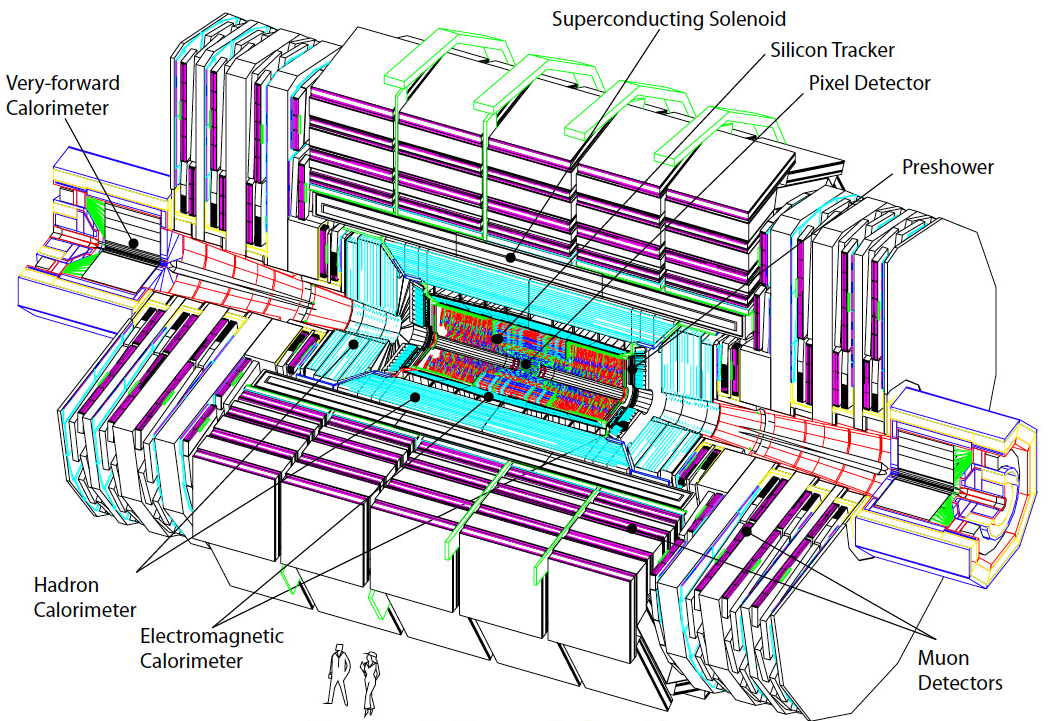
\includegraphics[width = 0.8 \textwidth]{Chapters/Chapter2_CERN/Figures/cms.png} \\ %Taken from http://inspirehep.net/record/884672/files/cms.png
 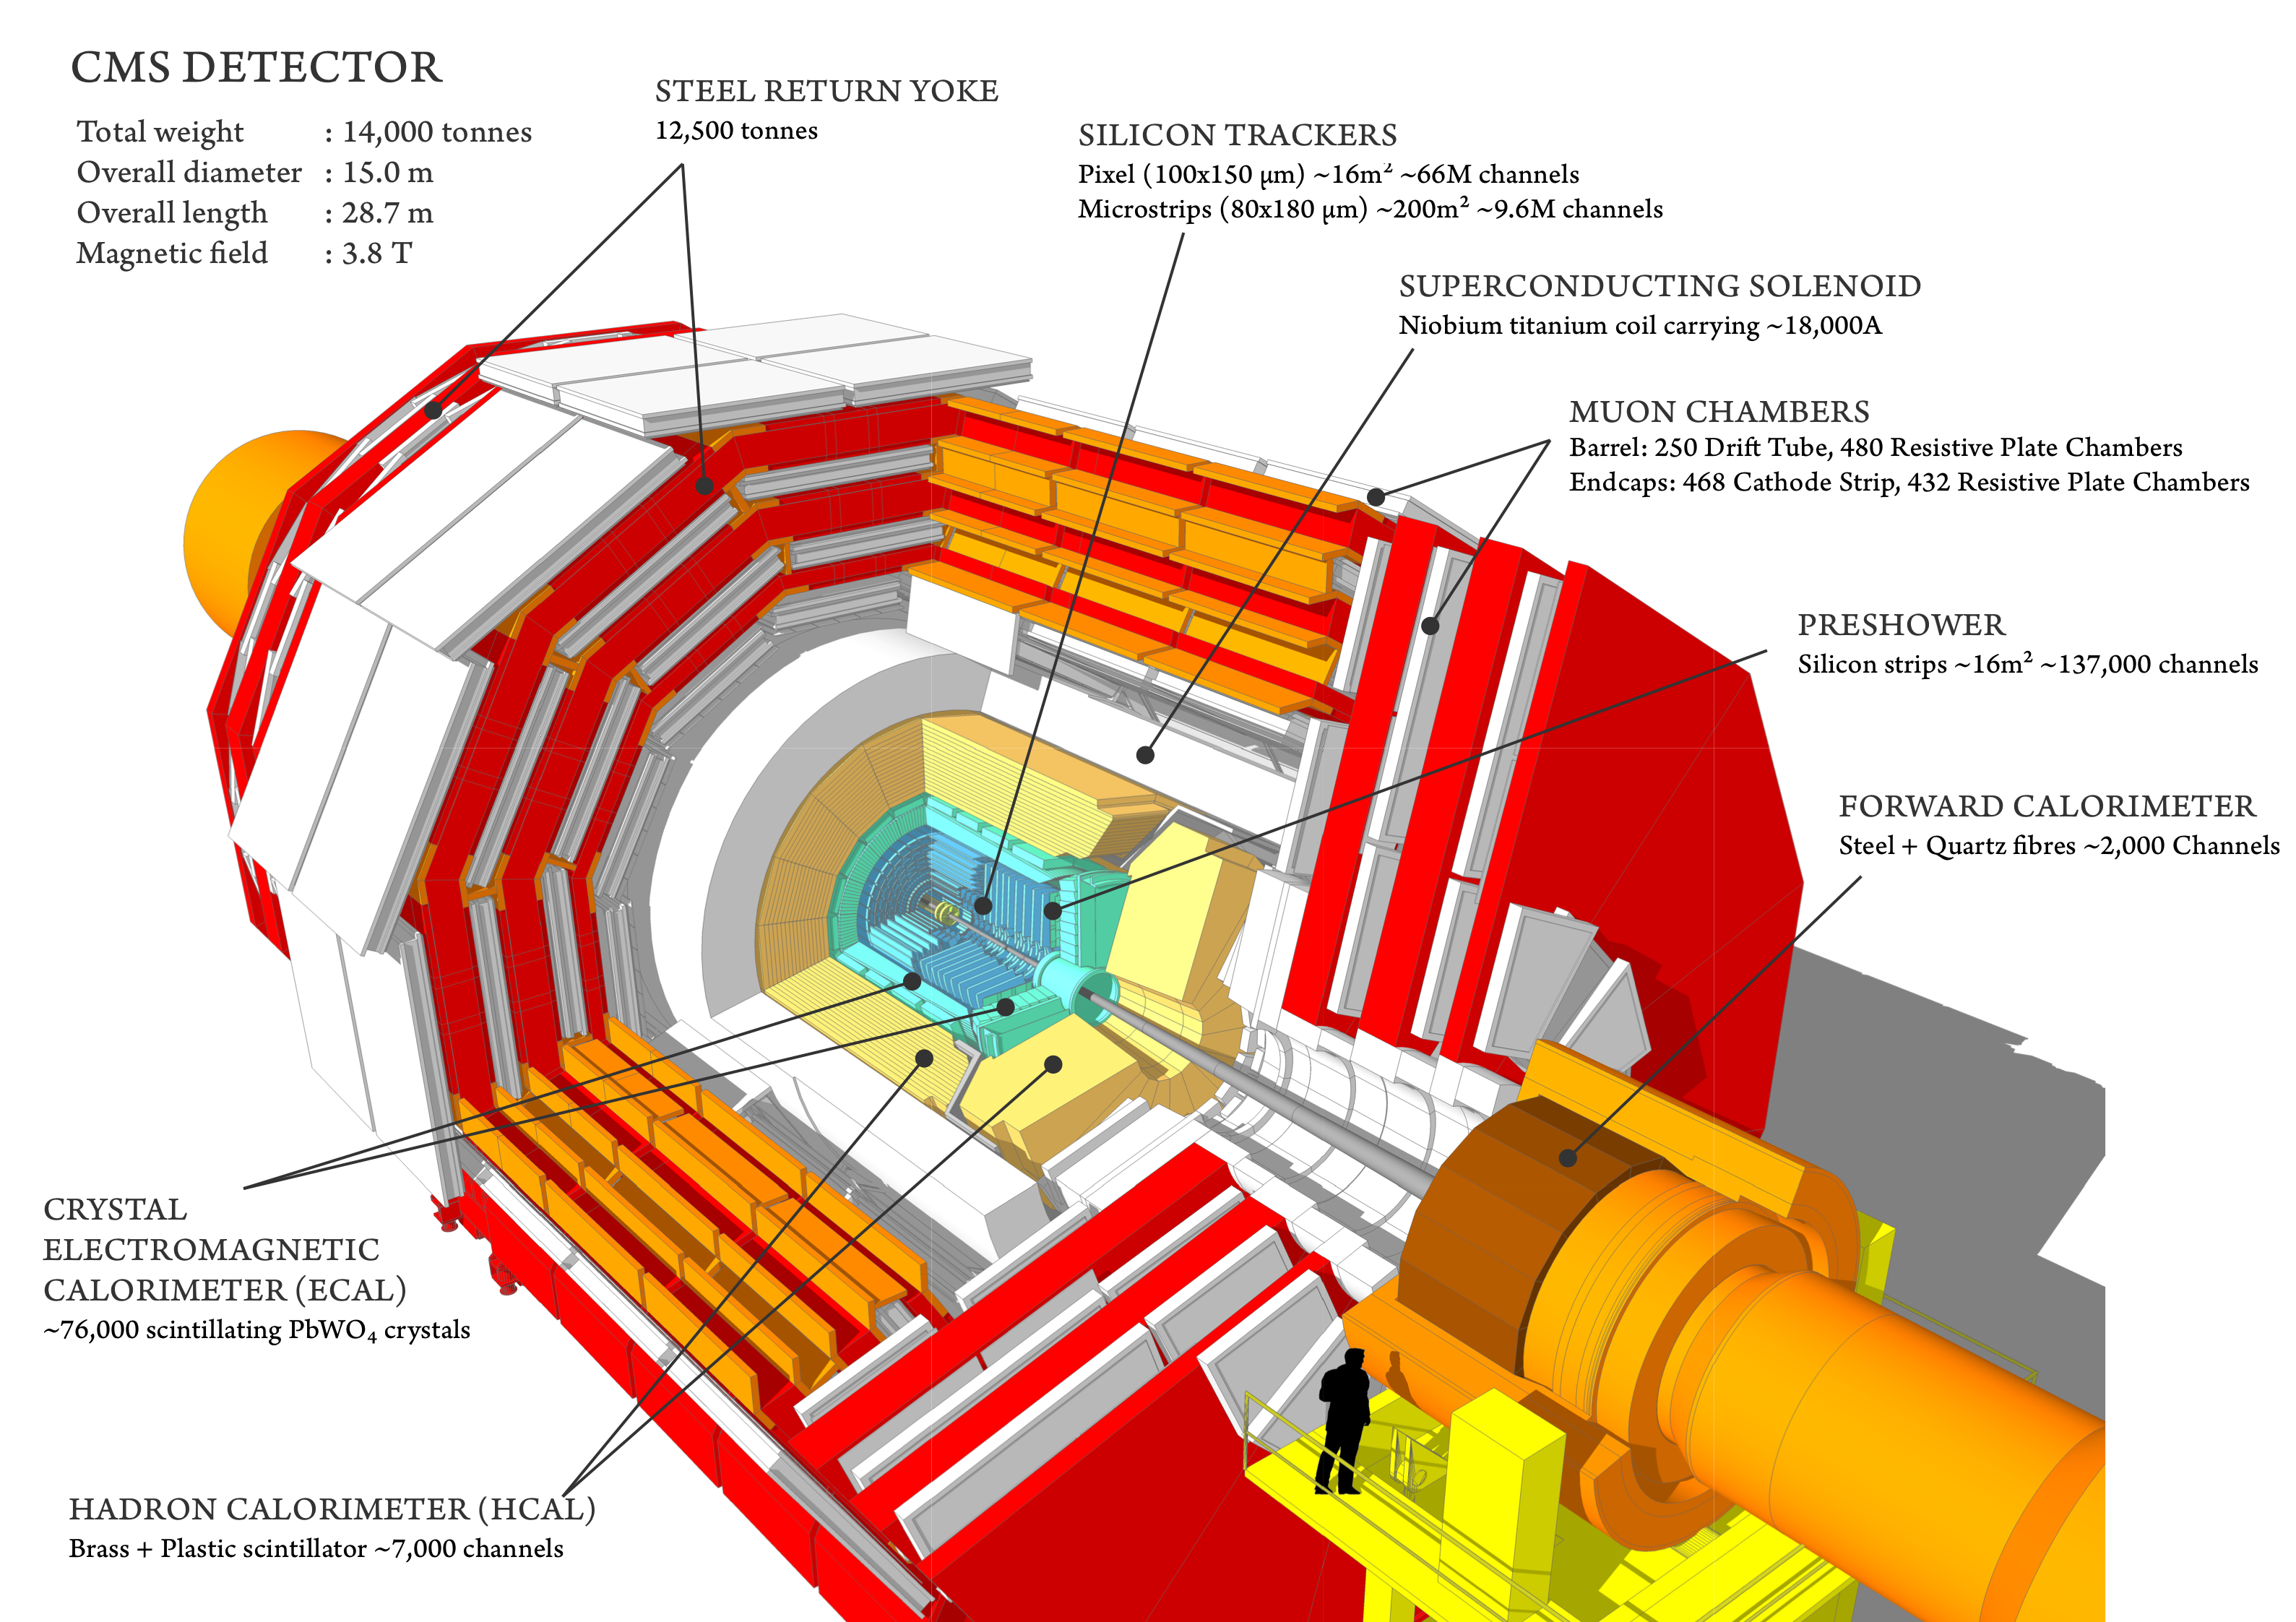
\includegraphics[width = 0.8 \textwidth]{Chapters/Chapter2_CERN/Figures/cms_MuchText.png}%Taken from https://cms-docdb.cern.ch/cgi-bin/PublicDocDB/RetrieveFile?docid=11514&version=1&filename=cms_120918_03.png
 \caption{CMS Figure with all subdetectors clearly visible} \label{fig::CMSFig}
\end{figure}

The design of the CMS experiment is \textbf{also} optimized for the reconstruction of neutrino's, which cannot be measured directly and hence only appear in the form of missing energy, by ensuring a hermetically closed detector. This resulted\footnote{Is this really the motivation why a barrel and endcap design has been adopted??} in the construction of a cylindrical barrel part located centrally with respect to the interaction point and an endcap part represented by a sort of disklike closure componenents for each of the different subdetectors.
Even though the CMS experiment is denominated as ``compact'', its overal dimensions are a total length of $21.6$ m and a diameter of $14.6$ m resulting in a total weight of $12500$ tons.

The CMS experiment has adopted a proper coordinate system for which the origin is centered at the nominal collision point within the detector. The $y$-axis (ordinate) is pointing upwards and the $x$-axis (abscissa) radially inwards toward the center of the LHC. Hence, according to the right-hand rule, the $z$-axis follows along the anticlockwise-beam direction. This coordinate system can easily be converted into a spherical coordinate system where the azimuthal angle $\phi$ is measured in the $x$-$y$ plane and the polar angle $\theta$ from the $z$-axis. 
A very important variable, which is used widely in accelerator physics, can now be derived from this coordinate system. The pseudorapidity $\eta$ is used to describe the angle of a particle with respect to the beam axis (or the $z$-axis) and is defined in Equation (\ref{eq::PseudoRapidity}). The key reason why this variable is so crucial in particle detectors is its invariance with respect to Lorentz boosts along the beam axis.

\begin{equation} \label{eq::PseudoRapidity}
 \eta = - \ln \tan \frac{\theta}{2}
\end{equation}

Another variable that is closely related is the rapidity, also denoted using the symbol $y$. Since this variable needs both the energy and total momentum of a particle it is much more challenging to correctly determine, but in the case of high energy collisions both quantities are almost identical.

\begin{equation}
 y = \frac{1}{2} \ln \left( \frac{E+p_{z}c}{E - p_{z}c} \right)
\end{equation}

\subsection{The silicon tracking apparatus}

\subsubsection*{Hit and track reconstruction in the pixel and strip tracker}

The tracking detector is responsible for translating the measured energy deposits in the pixel and strip tracker into charged particles' tracks. This process is done using a computationally challenging track reconstruction algorithm which proceeds in an iterative manner in order to first identify the straightforward prompt tracks.
The dense environment in the inner tracker is the main challenge for the track reconstruction implying the need of an efficient search for hits during the pattern recognition stage and a fast propagation of trajectory candidates. Hence the use of a Combinatiorial Track Finder (CTF), an extension of the Kalman Filter technique which allows the combination of track fitting and pattern recognition.

The local reconstruction is performed prior to the iterative tracking and clusters energy deposits by combining neighbouring pixels or strips which fullfill specific signal over noise (S/N) requirements. The cluster position is determined from the charge-weighted average or from the cluster edges in the case of the strip or pixel detector, respectively.

The track reconstruction algorithm can be decomposed into four separate steps: seed generation, pattern recognition, ambiguity resolution and track fitting.
The benefit of using an iterative process is that during the first iteration the easist to find tracks are identified such that their associated hits can be removed from the list in order to reduce combinatorial complexity for the following iterations.

\begin{myindentpar}
  \begin{description}
    \item[Seed generation] \hfill \\
    This step of the track reconstruction provides initial trajectory candidates from pairs of pixel hits. The track finding starts from trajectory seeds created in the innermost region of the tracker because the high granularity of the pixel detector ensures lower channel occupancy in the inner pixel layer than in the outer strip layer. 
    %Hence optimal efficiency is retrieved when the tracks are built in the outward direction.
    The starting trajectory parameters and their uncertainty in the quasi-uniform magnetic field of the tracker can be determined from five parameters. Hence either three 3-D hits or two 2D-hits combined with a beam spot constraint should be extracted in order to construct the seed trajectory.
    \item[Pattern recognition] \hfill \\
    This module of the CTF algorithm is basically a Kalman Filter which proceeds iteratively from the seed layer until the outermost tracker layer is reached. % taking into account the effects of multiple scattering and energy loss. 
    %Combining the information of successive layers significantly improves the precision of the track parameters for each layer. 
    First a dedicated navigation (step) is performed in order to identify the layers possibly intersected by the trajectory of the seed. Then, for each hit on this layer, a new trajectory candidate is created and its track parameters are recalculated using the Kalman Fiter formalism by combining the predicted trajectory state with the added hits in a weighted mean.
    \item[Ambiguity resolution] \hfill \\
    Since the track of a single charged particle can be reconstructed more than once, either originating from different seeds or when one single seed resulted in more than one trajectory candidate, double-counting is possible and should be resolved. Hence exclusion of specific tracks is performed based on the number of hits shared between two trajectories. 
    %The track with the fewest hits is removed and the trajectory cleaner is applied again on the remaining list of trajectory candidates. 
    \item[Track fitting] \hfill \\
    During the final step of the iterative tracking process the trajectory parameters are refitted using all hits in order to exclude any bias introduced during the seeding stage. The Kalman Filter used here starts from the innermost hit and proceeds outwards. Afterwards a so-called smoothing stage is applied in the form of an outside-in Kalman Fitler which uses the result of the first one. This approach yields optimal estimates of the parameters.
  \end{description}
\end{myindentpar}

%\textit{? Is this hit reconstruction (with fast and template-based algorithms) relevant?}

%The energy deposits detected in the pixel and strip tracker will be translated into actual charged particles' tracks by a track reconstruction algorithm. This is a computationally challenging tasks which is performed by a Combinatorial Track Finder (CTF), an extension of the Kalman Filter technique allowing the combined use of track fitting and pattern recognition. The process is performed iteratively, where each iteration proceeds in a similar manner:
%\begin{itemize}
% \item \textbf{Seed generation} \\
% During the first step of the CTF algorithm initial track candidates are identified which will serve as starting point for the reconstruction of the actual track parameters. The five parameters needed for representing the particle's trajectory in the tracker's magnetic field are retrieved by either three 3-D hits or two 2D-hits combined with a beam-spot constraint. The search for the seeds starts from the most inner layers of the pixel detector for efficiency optimization.
% \item \textbf{Track finding} \\
% In this step an inside-out Kalman Filter is applied in order to identify hits in successive detector layers compatible with the trajectory seed. After each layer the track parameters are updated taking into account the effects of multiple scattering and energy loss. This iterative process continues until the outermost layer of the tracker has been reached.
% \item \textbf{Track fitting} \\
% In order to obtain the most optimal track parameters, including the 
% \item \textbf{Track selection} \\
%\end{itemize}

\subsection{The calorimetry subdetectors}

\subsection{The muon system}

\subsection{Trigger and data acquisition}
